\chapter{Experimental Confirmation of the Photon}
\setcounter{section}{4}
\setcounter{subsection}{0}
\setcounter{subsubsection}{1}
\setcounter{secnumdepth}{3}
\setlength{\parindent}{0pt}
% Box styles
\tcbset{physikbox/.style={colback=blue!5!white, colframe=blue!75!black, fonttitle=\bfseries}}
\tcbset{mathebox/.style={colback=green!5!white, colframe=green!50!black, fonttitle=\bfseries}}
\tcbset{didaktikbox/.style={colback=yellow!5!white, colframe=yellow!50!black, fonttitle=\bfseries}}
\tcbset{hypobox/.style={colback=orange!5!white, colframe=orange!75!black, fonttitle=\bfseries}}
\tcbset{hinweisbox/.style={colback=gray!10!white, colframe=black!40!black, fonttitle=\bfseries}}

\subsection{The Photoelectric Effect}\index{Photoelectric Effect}

\subsubsection{Introduction and Classical Expectation}\index{Classical Electrodynamics}\index{Wave Model}

The so-called photoelectric effect – the emission of electrons from a metal surface when irradiated with light – was already known in the 19th century. Heinrich Hertz\index{Hertz, Heinrich} discovered the phenomenon in 1887 by accident during his investigations of electromagnetic radiation. Philipp Lenard\index{Lenard, Philipp} later studied it systematically and found: electrons are released from the metal when exposed to certain kinds of light.

Classical electrodynamics explained this behavior using the wave model of light\index{Wave Model}. According to that model, the energy of light should be transferred continuously to the electron via the electric field strength. From this, three seemingly plausible expectations followed:

\begin{itemize}
	\item \textbf{Intensity decides:} The higher the light intensity, the more energetic the emitted electrons should be.
	\item \textbf{Delay:} With weak light, a measurable time should pass until an electron has absorbed enough energy to be emitted.
	\item \textbf{Any wavelength possible:} In principle, any wavelength of light – even long-wave red light – should trigger electron emission if it is only intense enough.
\end{itemize}

These expectations seemed logical within the classical theory. But reality drastically contradicted them – a turning point in the history of physics.

\vspace{1em}
\begin{tcolorbox}[physikbox, title=Philipp Lenard (1902)\textit{ \cite{lenard1902} }]
	\label{box:Philipp Lenhard}
	
	\small
	“It turned out that light seemed to act with greater energy on electrons the shorter its wavelength was – regardless of how bright it was.”
\end{tcolorbox}

\subsubsection{Experimental Observations}

The systematic investigation of the photoelectric effect by Philipp Lenard\index{Lenard, Philipp}, Robert Millikan\index{Millikan, Robert A.}, and others led to observations that could not be reconciled with the classical wave theory. The central findings were:

\begin{itemize}
	\item \textbf{Immediate emission:} Electrons are released without measurable delay – even at extremely low light intensities.
	\item \textbf{Frequency dependence:} There exists a \emph{threshold frequency} \( \nu_{\text{min}} \)\index{Threshold Frequency}, below which no electrons are emitted – regardless of intensity.
	\item \textbf{Energy independent of intensity:} The kinetic energy of the emitted electrons depends solely on the frequency of the light – not on its intensity.
	\item \textbf{Linear relationship:} The electron energy increases linearly with the light frequency:
	\[
	E_{\text{kin}} = h \nu - A
	\]
	\index{Einstein Equation (Photoelectric Effect)}\index{Work Function}
\end{itemize}
(A more detailed derivation of Einstein’s equation for the photoelectric effect can be found in Appendix~A, Section~\ref{anhangA:photoeffekt}.)

These results fundamentally contradicted the classical expectation of continuous energy absorption from the electromagnetic field.

\vspace{1em}
\begin{tcolorbox}[physikbox, title=Albert Einstein (1905)\textit{ \cite{einstein1905}}]
	\label{die Erzeuguung von Licht}
	\small
	“The generation of light does not occur uniformly across the wavefront, but only at specific places, at individual points.”
\end{tcolorbox}
\index{Einstein, Albert}

\vspace{1em}
\begin{tcolorbox}[physikbox, title=Robert A. Millikan (1916)\textit{ \cite{millikan1916}}]
	\label{box:Robert A, Millikan}
	\small
	“Although I confirmed Einstein’s equation through years of experiments, I long resisted the idea that light consists of particles.”
\end{tcolorbox}
\vspace{1em}
\index{Millikan, Robert A.}

\textbf{Conclusion:} The observations could only be explained by assuming that light consists of discrete quanta – \emph{photons}\index{Photon}\index{Light Quantum|see{Photon}} – transferring their energy to an electron in a single collision. The classical wave picture had to be abandoned or profoundly modified.

\subsubsection{Einstein’s Explanation (1905)}\index{Einstein, Albert}\index{Light Quantum|see{Photon}}\index{Photon}\index{Heuristic Viewpoint (Einstein 1905)}

In 1905 Albert Einstein published his groundbreaking paper entitled \textit{“On a Heuristic Point of View Concerning the Production and Transformation of Light”} \cite{einstein1905}. In it he fundamentally questioned the classical idea of light as a continuous wave.\index{Classical Electrodynamics}\index{Wave Model}

Einstein proposed that light consists of individual energy portions – so-called \textbf{light quanta}\index{Light Quantum|see{Photon}}. These quanta carry a definite amount of energy:

\[
E = h \nu
\]\index{Planck–Einstein Relation@$E=h\nu$}

(A formal representation of the Planck–Einstein relation can be found in Appendix~A, Section~\ref{anhangA:planckEinstein}.)

A photon with frequency \( \nu \) thus possesses a discrete energy proportional to frequency. This idea was revolutionary, as it assigned a \emph{particle character} to light – contrary to the well-established Maxwell theory.\index{Maxwell, James Clerk}\index{Maxwell Theory}

Einstein further postulated that such a light quantum could transfer its energy completely to an electron in a collision. 

Only if the energy of the photon is greater than the so-called \textbf{work function} \( A \), an electron is released from the metal:\index{Work Function}

\[
E_{\text{kin}} = h \nu - A
\]\index{Einstein Equation (Photoelectric Effect)}

This equation explains directly:
\begin{itemize}
	\item Why only light of sufficiently high frequency can release electrons,
	\item Why emission occurs immediately (a single photon suffices),
	\item Why the kinetic energy of electrons grows linearly with frequency.
\end{itemize}

Einstein’s explanation was radical – and at first highly controversial. Even Max Planck, the founder of quantum theory, considered the light quantum hypothesis too speculative.\index{Planck, Max}

\vspace{1em}
\begin{tcolorbox}[physikbox, title=Albert Einstein (1905)\textit{ \cite{einstein1905}}]
	\label{die Erscheinung der Wärm}
	\small
	“The phenomena of thermal radiation demand a viewpoint according to which light consists of discrete quanta of energy in the direction of propagation.”
\end{tcolorbox}
\index{Einstein, Albert}
\vspace{1em}
\textbf{Assessment:} Einstein turned Planck’s mathematical trick into physical reality. With this he laid the foundation for the modern concept of the photon and the quantized nature of the electromagnetic field.\index{Photon}\index{Quantized Electromagnetic Field}

\subsubsection{Millikan’s Measurements (1916)}\index{Millikan, Robert A.}

Although Einstein’s light quantum hypothesis provided a convincing explanation for the photoelectric effect, it was initially heavily disputed. Many physicists – including Max Planck – considered it unimaginable that light should consist of real particles.\index{Planck, Max} One of the most prominent skeptics was \textbf{Robert A. Millikan}.\index{Millikan, Robert A.}

In a series of experiments (1909–1916), Millikan developed a particularly precise setup to systematically test Einstein’s equation. Using a vacuum photo cell\index{Vacuum Photocell}, finely adjustable counter voltages\index{Counter Voltage}, and monochromatic light sources\index{Monochromatic Light}, he was able to directly measure the maximum kinetic energy of the electrons at different light frequencies.

\textbf{The result:} Despite all his doubts, Millikan found a crystal-clear confirmation of Einstein’s prediction:

\[
e U = h \nu - A
\]\index{Einstein Equation (Photoelectric Effect)}\index{Work Function}

(A detailed derivation of the stopping voltage equation and its experimental significance can be found in Appendix~A, Section~\ref{anhangA:stoppspannung}.)

Here \( U \) is the counter voltage required to fully suppress the electron current. The slope of the resulting straight line (electron energy vs. frequency) yielded with high accuracy Planck’s constant \( h \).\index{Planck’s Constant@$h$ (Planck’s Constant)}

\vspace{1em}
\begin{tcolorbox}[physikbox, title=Robert A. Millikan (1916)\textit{ \cite{millikan1916}}]
	\label{box:einsteins gleichung passt}
	\small
	“Einstein’s equation matches the data with astonishing accuracy – and yet I cannot bring myself to regard it as theoretically satisfying.”
\end{tcolorbox}
\index{Millikan, Robert A.}
\vspace{1em}

\textbf{Remarkable:} With utmost precision, Millikan disproved the classical theory – and confirmed Einstein’s light quantum – but was reluctant to accept the concept. Only years later did he recognize the quantized nature of light as physical reality.

\textbf{Significance:} Millikan’s measurements are considered one of the most important experimental proofs of the photon concept.\index{Photon} They strengthened the acceptance of Einstein’s theory – although it was only fully appreciated with the development of quantum mechanics.\index{Quantum Mechanics}

\subsubsection{Mathematical Description}\index{Einstein Equation (Photoelectric Effect)}\index{Work Function}

The central formula for describing the photoelectric effect is based on Einstein’s assumption that each photon possesses a discrete energy \( E = h\nu \).\index{Planck–Einstein Relation@$E=h\nu$} When such a photon hits an electron in the metal, its energy is transferred to the electron. The energy balance is:

\[
E_{\text{Photon}} = E_{\text{Work Function}} + E_{\text{kin}}
\quad\Rightarrow\quad h \nu = A + E_{\text{kin}}
\]\index{Einstein Equation (Photoelectric Effect)}


Where:

- \( h \) is Planck’s constant\index{Planck’s Constant@$h$ (Planck’s Constant)}  
- \( \nu \) is the frequency of the incident light\index{Frequency}  
- \( A \) is the material-dependent \textbf{work function}\index{Work Function}  
- \( E_{\text{kin}} \) is the kinetic energy of the electron\index{Kinetic Energy}

If a counter voltage \( U \) is applied to suppress the electron current, then the energy \( e U \) corresponds to the maximum kinetic energy of the electrons:\index{Counter Voltage}\index{Stopping Voltage@Stopping Voltage (Photoelectric Effect)}

\[
eU = h \nu - A
\]\index{Einstein Equation (Photoelectric Effect)}

This is the experimentally measurable form of Einstein’s equation.

\vspace{0.5em}
\begin{tcolorbox}[physikbox, title=What is the Work Function \( A \)?]
	\label{bos:was ist Austrittsarbeit}
	\small
	The work function \( A \) is the minimum energy required to release an electron from the metal. It depends on the material and typically lies between 2\,eV (e.g. cesium) and 5\,eV (e.g. platinum). Only if \( h \nu > A \), an electron is emitted.
\end{tcolorbox}
\vspace{1em}

\textbf{Graphical representation:}\index{Stopping Voltage@Stopping Voltage (Photoelectric Effect)}\index{Threshold Frequency}

The equation describes a \textit{linear dependence} of electron energy (or stopping voltage \( U \)) on frequency \( \nu \). The graph is a straight line:
\begin{figure}[H]
	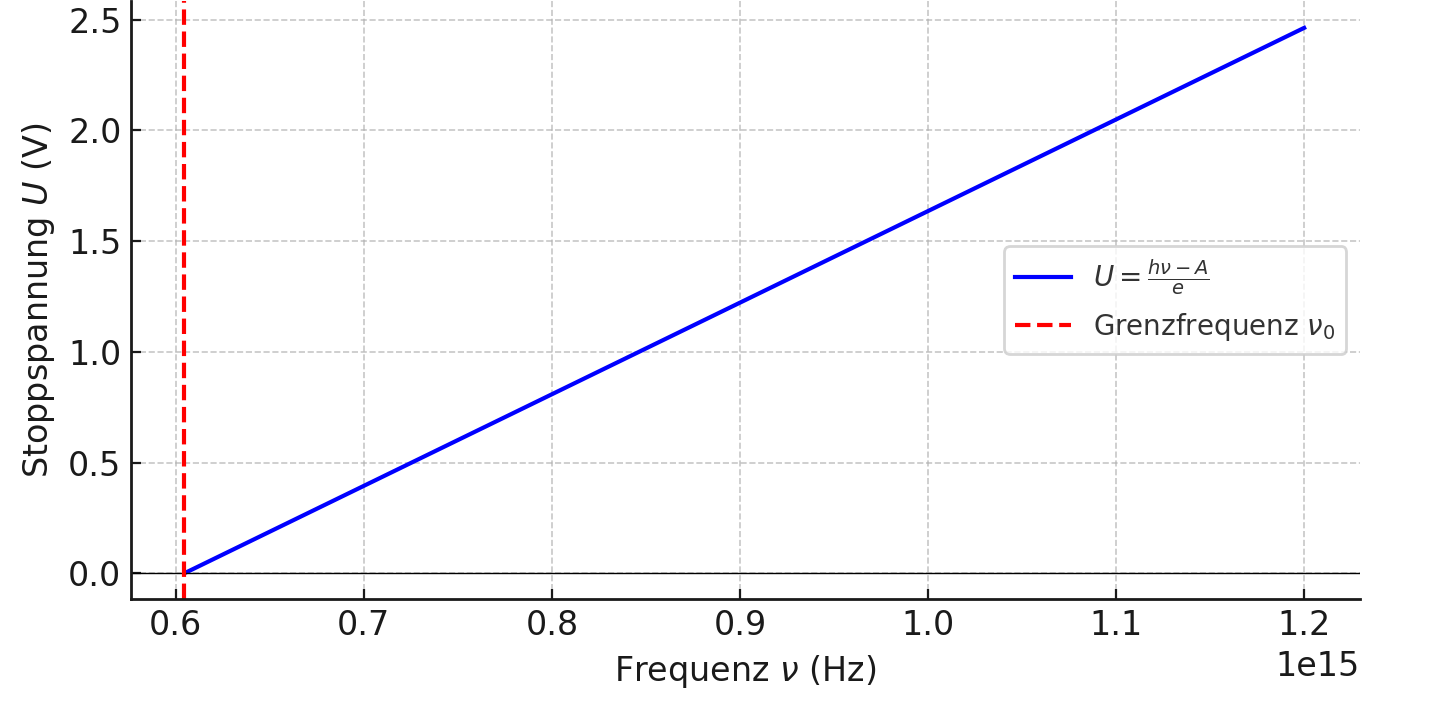
\includegraphics[width=0.65\textwidth]{bilder/photoeffekt.png}
	\caption{Linear dependence of electron energy on frequency.}
\end{figure}

\begin{itemize}
	\item The \textbf{slope} of the line corresponds to \( h/e \)
	\item The \textbf{x-intercept} \( \nu_0 \) is the threshold frequency: \( h \nu_0 = A \)\index{Threshold Frequency}
	\item For \( \nu < \nu_0 \) no emission occurs – regardless of intensity
\end{itemize}

This linear relationship was experimentally confirmed with high accuracy by Millikan.\index{Millikan, Robert A.}

\textbf{Consequence:}

\begin{quote}
	The energy of a photon depends solely on its frequency – not on light intensity.
\end{quote}
\index{Frequency}\index{Intensity}

\subsubsection{Comparison: Wave Model vs. Photon Model}\index{Wave Model}\index{Photon Model}\index{Wave–Particle Duality@Wave–Particle Duality (Contrast)}

Explaining the photoelectric effect marked a profound paradigm shift in physics: from the classical wave picture of light to a quantized particle model.\index{Paradigm Shift} To illustrate the significance of this change, it is useful to directly compare both models.

\vspace{1em}
\begin{table}[H]
	\centering
	\begin{tabular}{|p{4.75cm}|p{4.75cm}|}
		\hline
		\textbf{Classical Wave Model} & \textbf{Photon Model (Einstein)} \\
		\hline
		Light is a continuous wave in the electromagnetic field & Light consists of individual quanta (photons) with energy \( E = h\nu \) \\
		\hline
		Energy is transferred continuously via field strength & Energy is transferred abruptly in discrete portions \\
		\hline
		Intensity determines the energy transfer & Intensity only determines the \emph{number} of photons, not their energy \\
		\hline
		Any frequency can release electrons if intensity is high enough & Only photons with \( h\nu > A \) release electrons \\
		\hline
		Energy is accumulated slowly; time delay possible & Immediate emission when a photon strikes \\
		\hline
	\end{tabular}
	\caption{Comparison between the classical wave model and Einstein’s photon model for the photoelectric effect}
	\label{tab:vergleich_photoeffekt}
\end{table}

\vspace{1em}

\begin{tcolorbox}[didaktikbox, title=Didactic Clarification]
	\label{box:didaktischeKlarstellung}
	\small
	In the wave model, light intensity determines the strength of energy transfer – in the photon model, however, it only determines the number of incident quanta.\\
	The energy of an individual photon depends exclusively on frequency.
\end{tcolorbox}
\vspace{1em}
\index{Intensity}\index{Frequency}\index{Photon}

\textbf{Typical Misunderstanding:}  
“Bright light must release more energetic electrons.”  
$\rightarrow$ \emph{False}, because with light below the threshold frequency nothing happens – regardless of brightness.\index{Threshold Frequency}

\textbf{Assessment:}  
The photoelectric effect was the first direct proof that electromagnetic radiation has not only wave character, but also particle properties. This duality was later generalized in the concept of wave–particle duality.\index{Wave–Particle Duality}

\subsubsection{Significance for Physics}\index{Photoelectric Effect!Significance}\index{Photon}\index{Quantized Nature of Light}\index{Einstein, Albert}\index{Classical Electrodynamics}

The photoelectric effect was the first phenomenon that could only be explained by assuming a quantized nature of light. Einstein’s light quantum hypothesis of 1905 contradicted classical electrodynamics and was initially dismissed as speculative. But Millikan’s precise confirmation in 1916 forced the scientific community to fundamentally rethink the concept of light.\index{Millikan, Robert A.}

\textbf{Physical Consequences:}
\begin{itemize}
	\item Energy transfer of light does not occur continuously, but in discrete quanta – the photons.\index{Photon}
	\item The energy of a photon is proportional to frequency: \( E = h\nu \).\index{Planck–Einstein Relation@$E=h\nu$}\index{Frequency}
	\item The photoelectric effect provided the first direct experimental proof of this quantization.\index{Photoelectric Effect!Proof}
\end{itemize}

Einstein himself received the Nobel Prize in 1921 – explicitly not for relativity, but:\index{Nobel Prize!Einstein 1921}\index{Theory of Relativity}
\begin{quote}
	“for his services to theoretical physics, and especially for his discovery of the law of the photoelectric effect.”
\end{quote}

Millikan was also awarded the Nobel Prize in 1923 – for his determination of the elementary charge and his work on the photoelectric effect.\index{Nobel Prize!Millikan 1923}\index{Elementary Charge}

\vspace{1em}
\begin{tcolorbox}[hinweisbox, title=Conclusion]
	\label{box:fazit der photo}
	\small
	The photoelectric effect marks the beginning of the photon concept – and thus the dawn of quantum physics.\\
	It shows: light not only has wave properties, but under certain conditions behaves like a particle.
\end{tcolorbox}
\index{Quantum Physics}
\vspace{1em}

\textbf{Outlook:}  
In the next section we will consider another key experiment: \textbf{Compton scattering}. It demonstrates not only the energy transfer, but also the \emph{momentum transfer} of photons – a decisive proof of the particle character of light.\index{Compton Scattering}\index{Momentum Transfer}

\subsection{Compton Scattering}\index{Compton Scattering}\index{Compton, Arthur H.}\index{X-rays}

\subsubsection{The Compton Experiment (1923)}\index{Compton, Arthur H.!Experiment (1923)}

In 1923 the American physicist \textbf{Arthur H. Compton} published the results of a scattering experiment with X-rays that would revolutionize physics. He directed high-energy photons onto nearly free electrons – for example in graphite – and analyzed the scattered radiation as a function of angle.\index{Electron}\index{Graphite}

The central observation was striking: the scattered light had a longer wavelength (lower energy) than the incident light, and the wavelength shift depended systematically on the scattering angle.\index{Wavelength Shift}\index{Scattering Angle}

This change could not be explained by classical scattering (such as Thomson scattering) or interference. Compton interpreted the result as an \textbf{elastic collision} between a photon and an electron – fully in line with a particle model of light. Thus the photon was not only a carrier of energy, but also of momentum.\index{Thomson Scattering}\index{Elastic Collision}\index{Photon Momentum}

\textbf{Physical principle:}
\begin{itemize}
	\item A photon with wavelength \( \lambda \) strikes a stationary electron.
	\item During the collision the photon is deflected (scattering angle \( \theta \)) and transfers momentum and energy to the electron.
	\item The scattered photon has a new wavelength \( \lambda' > \lambda \).
\end{itemize}

\textbf{Key equation:}
\[
\Delta \lambda = \lambda' - \lambda = \frac{h}{m_e c}(1 - \cos \theta)
\]\index{Compton Formula}\index{Compton Wavelength}\index{Electron!Mass $m_e$}

\vspace{1em}
\begin{figure}[H]
	\begin{center}
		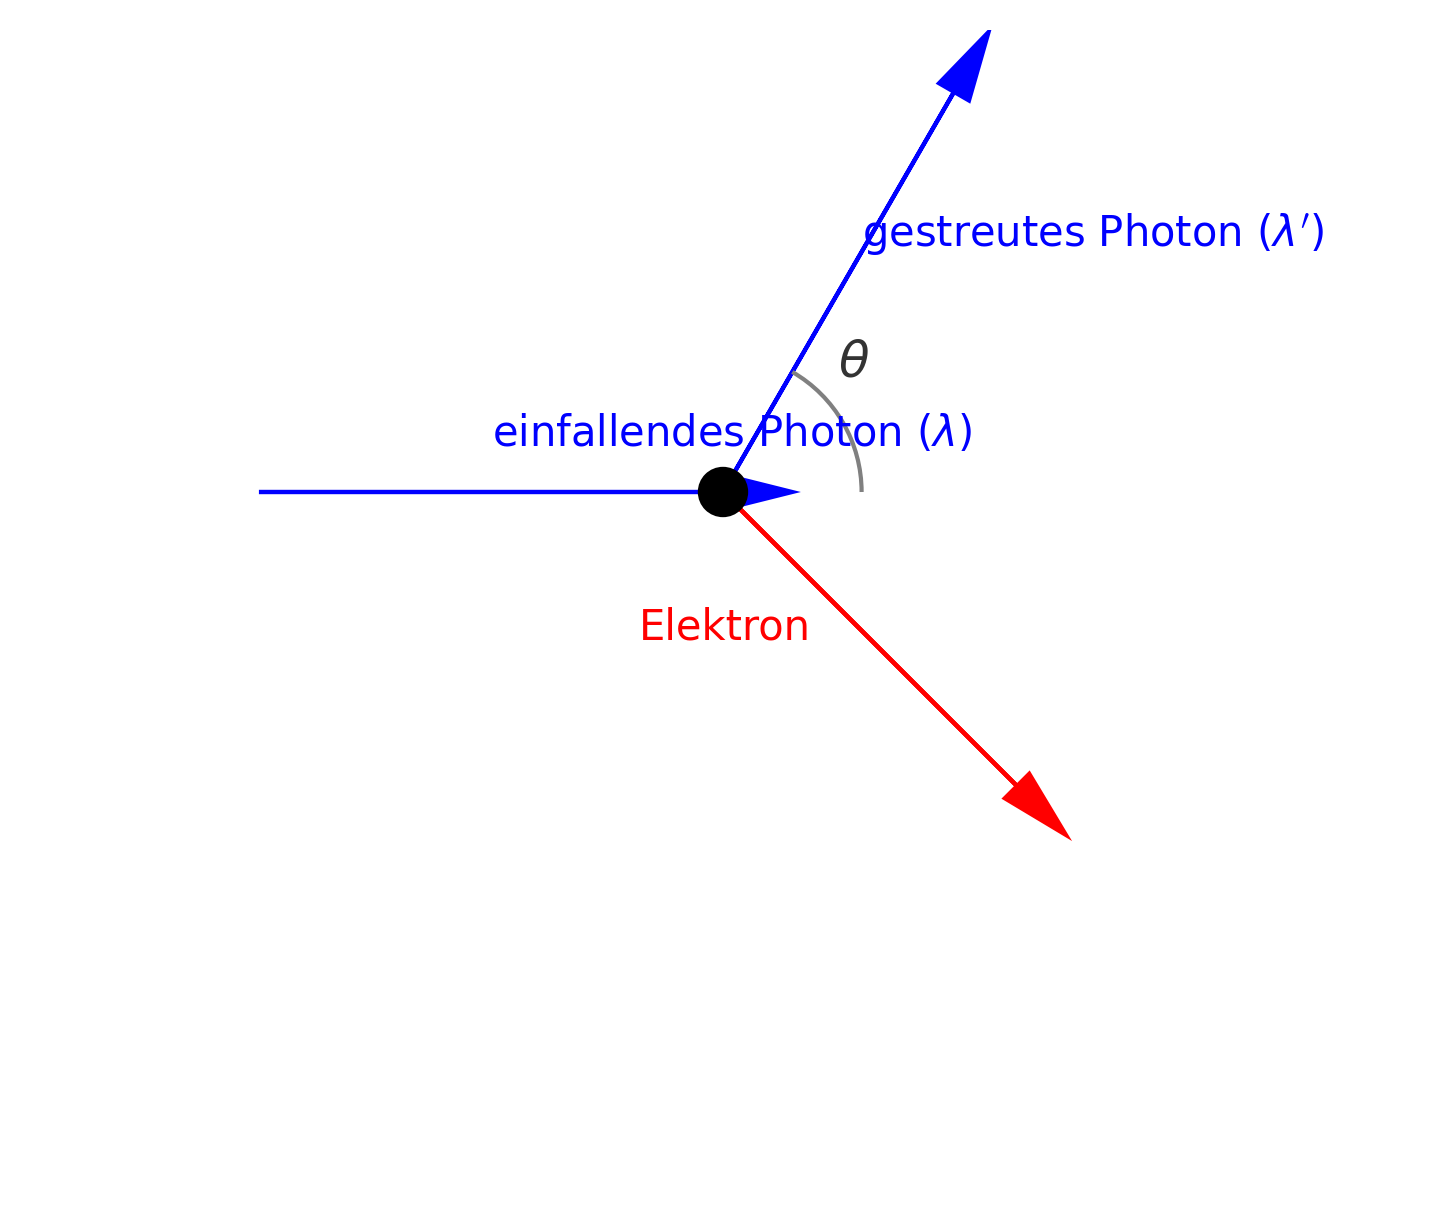
\includegraphics[width=0.6\textwidth]{bilder/compton-schema.png}
	\end{center}
	\caption{Schematic representation of Compton scattering: a photon transfers momentum to an electron.}
\end{figure}

\textbf{Significance:}  
Compton scattering was the first experimental proof that photons possess momentum – a decisive step toward accepting the photon as a real particle. Arthur Compton received the Nobel Prize in Physics in 1927 for this.\index{Photon Momentum}\index{Nobel Prize!Compton 1927}
\newpage
\noindent
\subsubsection{Compact Derivation of the Compton Formula}\index{Compton Formula!Derivation}\index{Energy Conservation}\index{Momentum Conservation}

The central observation in the Compton effect is: the scattered photon has a longer wavelength than the incident photon. This shift can only be explained if the photon is assigned not only energy \( E = h\nu \), but also momentum \( p = h/\lambda \).\index{Planck–Einstein Relation@$E=h\nu$}\index{Photon Momentum}

\textbf{Basic idea of the derivation:}  
A photon strikes a stationary electron. During the collision, energy and momentum are transferred to the electron. The situation resembles an elastic collision of two particles – with the difference that one of them is massless.\index{Elastic Collision}\index{Massless Particles}


\textbf{Core assumptions:}
\begin{itemize}
	\item \textbf{Energy conservation:} The sum of photon energy and electron rest energy is conserved.
	\item \textbf{Momentum conservation:} The momentum vectors before and after the collision must balance – in both x- and y-directions.
	\item \textbf{Photon momentum:} For the photon \( p = \frac{h}{\lambda} \), for the electron the relativistic energy–momentum relation applies.\index{Relativistic Energy–Momentum Relation}
\end{itemize}

Applying these conservation laws and simplifying yields the \textbf{Compton formula}:

\vspace{1em}
\begin{tcolorbox}[mathebox, title=Compton Formula]
	\label{box:comptonFormel}
	\small
	\[
	\Delta \lambda = \lambda' - \lambda = \frac{h}{m_e c}(1 - \cos \theta)
	\]
\end{tcolorbox}
\vspace{1em}
(A more detailed derivation of the Compton formula can be found in Appendix~A, Section~\ref{anhangA:comptonHerleitung}.) 

\textbf{Physical interpretation:}
\begin{itemize}
	\item The wavelength of the scattered photon increases with the scattering angle \( \theta \).\index{Scattering Angle}
	\item The factor \( \frac{h}{m_e c} \approx 2.43 \cdot 10^{-12}\,\mathrm{m} \) is known as the \emph{Compton wavelength} of the electron.\index{Compton Wavelength}
	\item The effect shows that the photon transfers \emph{momentum} – a clear proof of its particle character.\index{Photon Momentum}
\end{itemize}
\subsection{Double-Slit Experiment with Single Photons}\index{Double-Slit Experiment}\index{Single Photon}\index{Interference}\index{Wave–Particle Duality}

A central argument for the wave nature of light since the 19th century was the observation of interference patterns – in particular in the famous double-slit experiment. But modern experiments show: even single photons, sent one after another through the setup, produce an interference pattern on the screen. This is only explainable if the photon also possesses wave character.\index{Interference Pattern}


\textbf{Experimental setup:}
\begin{itemize}
	\item A weak light source emits single photons – so weak that never more than one is in the setup at the same time.\index{Single-Photon Source}
	\item The photons pass through two closely spaced slits (double slit).\index{Double Slit}
	\item Behind them is a light-sensitive screen or detector.\index{Detector}
\end{itemize}

\textbf{Observation:}
\begin{itemize}
	\item Each individual photon is registered as a point – like a particle.\index{Particle Aspect of Light}
	\item Over time, however, an interference pattern emerges – like a wave.\index{Wave Aspect of Light}
\end{itemize}

\vspace{1em}
\begin{figure}[H]
	\begin{center}
		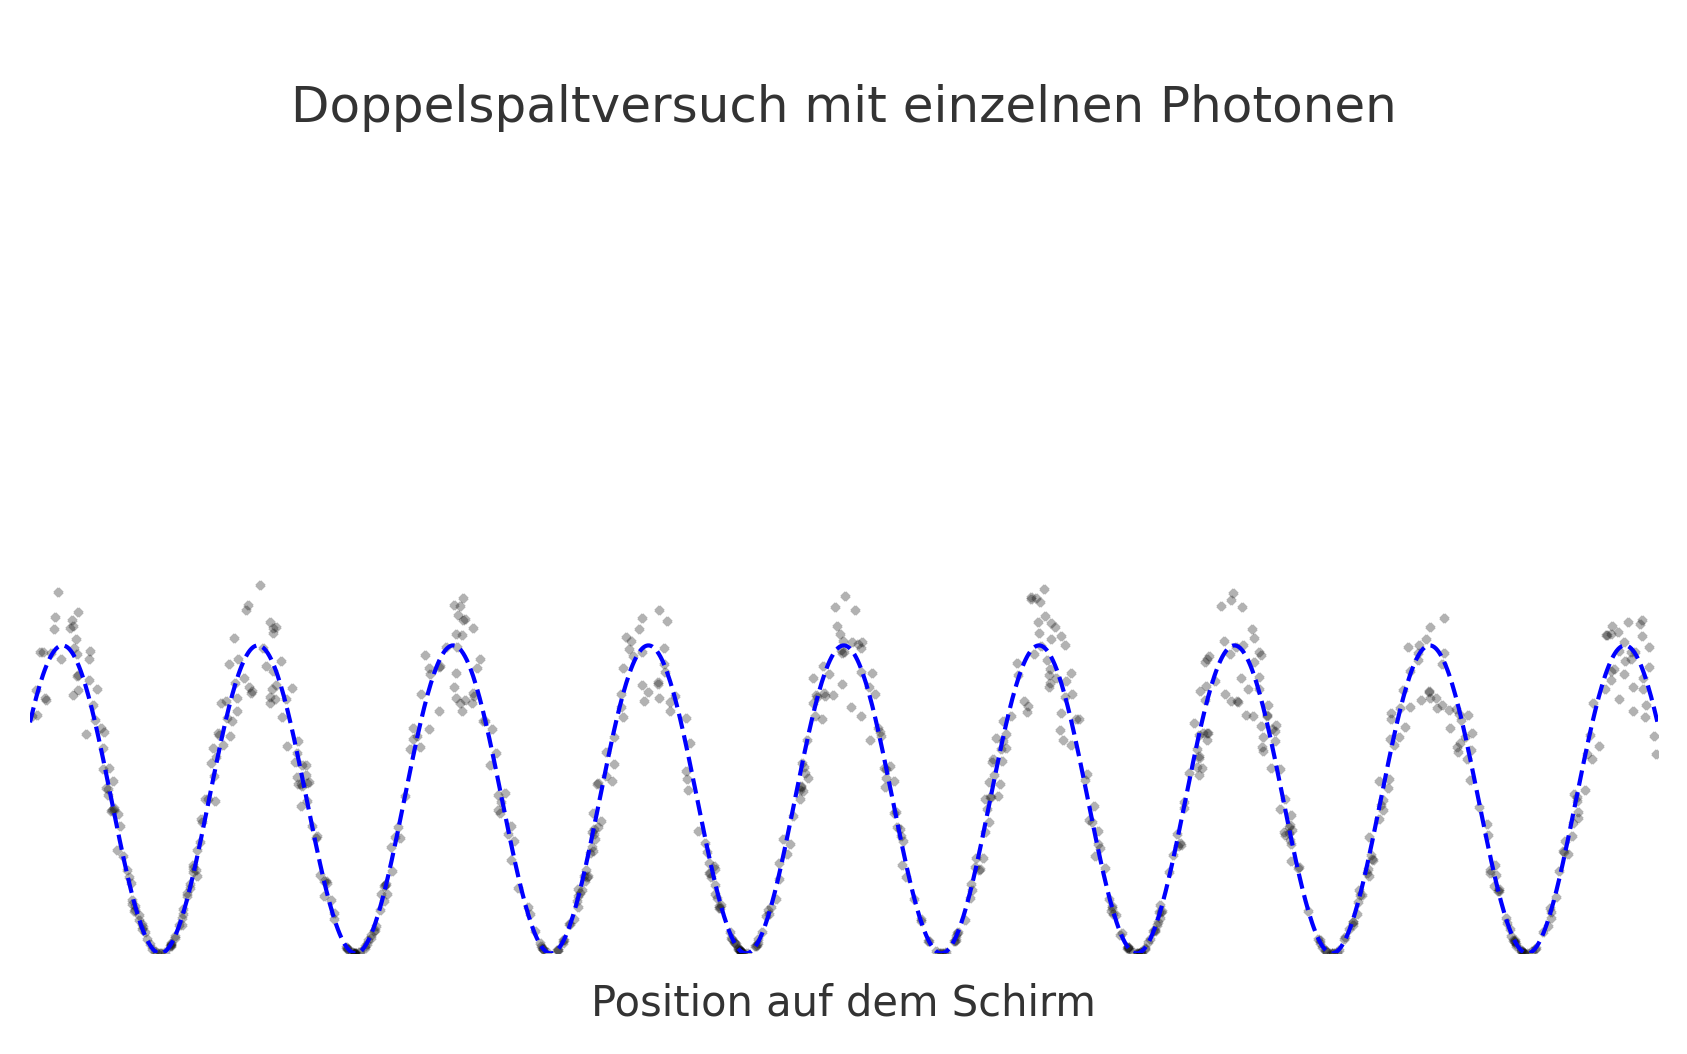
\includegraphics[width=0.65\textwidth]{bilder/doppelspalt-photonen.png}
	\end{center}
	\caption{Double-slit experiment with single photons: particle detections with a wave pattern.}
\end{figure}
\newpage
\noindent
\begin{tcolorbox}[physikbox, title=What the Photon Graphic is Meant to Show]
	\label{box:was die photonengrafik}
	\small
	\begin{itemize}
		\item The dots represent individual photon detections – the particle aspect of light.
		\item Over time a pattern emerges that is typical of wave interference – as with water waves.
		\item The dashed line shows only the statistical frequency of detection locations – it is not a light ray and not a real wave.
	\end{itemize}
\end{tcolorbox}
\vspace{1em}
(A mathematical formalization of the double-slit experiment with single photons and the superposition representation can be found in Appendix~A, Section~\ref{anhangA:doppelspalt}.) 

\textbf{Interpretation:}  
The photon apparently interferes with itself – it “passes through both slits simultaneously.” Only upon detection on the screen does the state collapse into a single event. This behavior can only be understood within quantum mechanics: the photon is neither a classical wave nor a classical particle – it exhibits both, depending on the experiment.\index{Self-Interference}\index{Quantum Mechanics}\index{Wavefunction Collapse}

\vspace{1em}
\begin{tcolorbox}[hypobox, title=Key Idea]
	\label{box:schlüsselidee}
	\small
	The double-slit experiment with single photons shows: the quantum nature of light encompasses both wave and particle properties. The interference pattern emerges even though never two photons are in the system at the same time.
\end{tcolorbox}
\vspace{1em}
\begin{tcolorbox}[didaktikbox, title=Wave as well as Particle Properties]
	\label{box:wellen}
	\small
	The interference pattern disappears immediately if one tries to determine the photon’s path through one of the slits. The possibility of interference is tied to the \emph{unknowability of the path} – a basic principle of quantum physics.
\end{tcolorbox}
\index{Which-Path Information}

\subsubsection*{Summary}\index{Double-Slit Experiment!Summary}\index{Superposition}

\phantomsection
\begin{tcolorbox}[didaktikbox, title=Conclusion: An Apparently Paradoxical Behavior]
	\label{box:Fazit ein scheinbarer}
	\small
	Even when photons are sent one by one – successively – through the double slit, an interference pattern emerges over time.
	
	This raises a profound question: How does a single photon “know” that it is part of a pattern?
	
	In classical terms there would have to be some kind of communication between photons – but that is not the case. Each photon seems to interfere with itself. Quantum mechanics explains this by the \textbf{superposition of all possible paths}: the photon has not gone through one or the other slit – but through both, as long as the path is not measured.
	
	This notion contradicts our everyday experience – but is experimentally beyond doubt. The double-slit experiment is therefore a key result of quantum physics.
	
	The double-slit experiment with single photons challenges our classical thinking:  
	How can a single photon contribute to building an interference pattern, although no second photon is present in the setup at the same time?
	
	Apparently each photon interferes with itself. In the language of quantum mechanics this means: as long as no measuring device determines the path, all possible paths are superposed – including “through both slits at once.”
	
	This superposition collapses only upon detection into a single point. The interference pattern arises not from interaction between photons, but from the \emph{statistics of many single measurements} – and from the quantum-mechanical structure of state space.
	
	What looks like “communication” is in fact an expression of the nonclassical nature of the quantum world.
\end{tcolorbox}

\subsection{Antibunching: The Proof of Single Photons}\index{Antibunching}\index{Single Photon}\index{Single-Photon Source}\index{Beam Splitter}\index{Detector}

A particularly convincing experimental proof for the existence of single photons is provided by the phenomenon of \textbf{antibunching}. Here a light source is used that emits only one photon at a time – for example, a fluorescing atom or a quantum dot.\index{Quantum Dot}\index{Fluorescence}

In a setup with a beam splitter and two detectors, it turns out: it \emph{never happens} that both detectors register a signal at the same time. This means: there is no such thing as “half a photon” – but always exactly one, which arrives either here or there.\\

\textbf{Why does this contradict the classical wave picture?} \\
In classical theory, light is a continuous electromagnetic wave. When such a wave strikes a beam splitter, it is \emph{divided}: one part goes left, the other right. Thus – at least with strong intensity – both detectors should sometimes register a signal simultaneously.\index{Classical Electrodynamics}\index{Wave Model}

In contrast, antibunching shows: \emph{never} are both detectors triggered at once. This means that the light does not arrive split, but in \textbf{indivisible energy packets} – single photons. This directly contradicts the classical wave picture.\index{Photon!Indivisibility}

\vspace{1em}
\begin{tcolorbox}[physikbox, title=What Antibunching Shows]
	\label{box:wasAntibunching}
	\small
	Light cannot be split into two directions simultaneously if it consists of single photons.\\
	This contradicts every classical wave picture – but precisely matches the behavior of indivisible light quanta.
\end{tcolorbox}
\vspace{1em}
(A mathematical description of the second-order correlation function \( g^{(2)}(0) \) can be found in Appendix~A, Section~\ref{anhangA:antibunching}.) 

\subsection{Hong–Ou–Mandel Effect: Interference of Two Photons}\index{Hong–Ou–Mandel Effect}\index{Photon Indistinguishability}\index{Probability Amplitude}\index{Beam Splitter}

Another striking experiment is the \textbf{Hong–Ou–Mandel (HOM) effect}. Two identical photons are sent from opposite directions onto a half-transparent mirror (beam splitter).

\begin{figure}[H]
	\begin{center}
		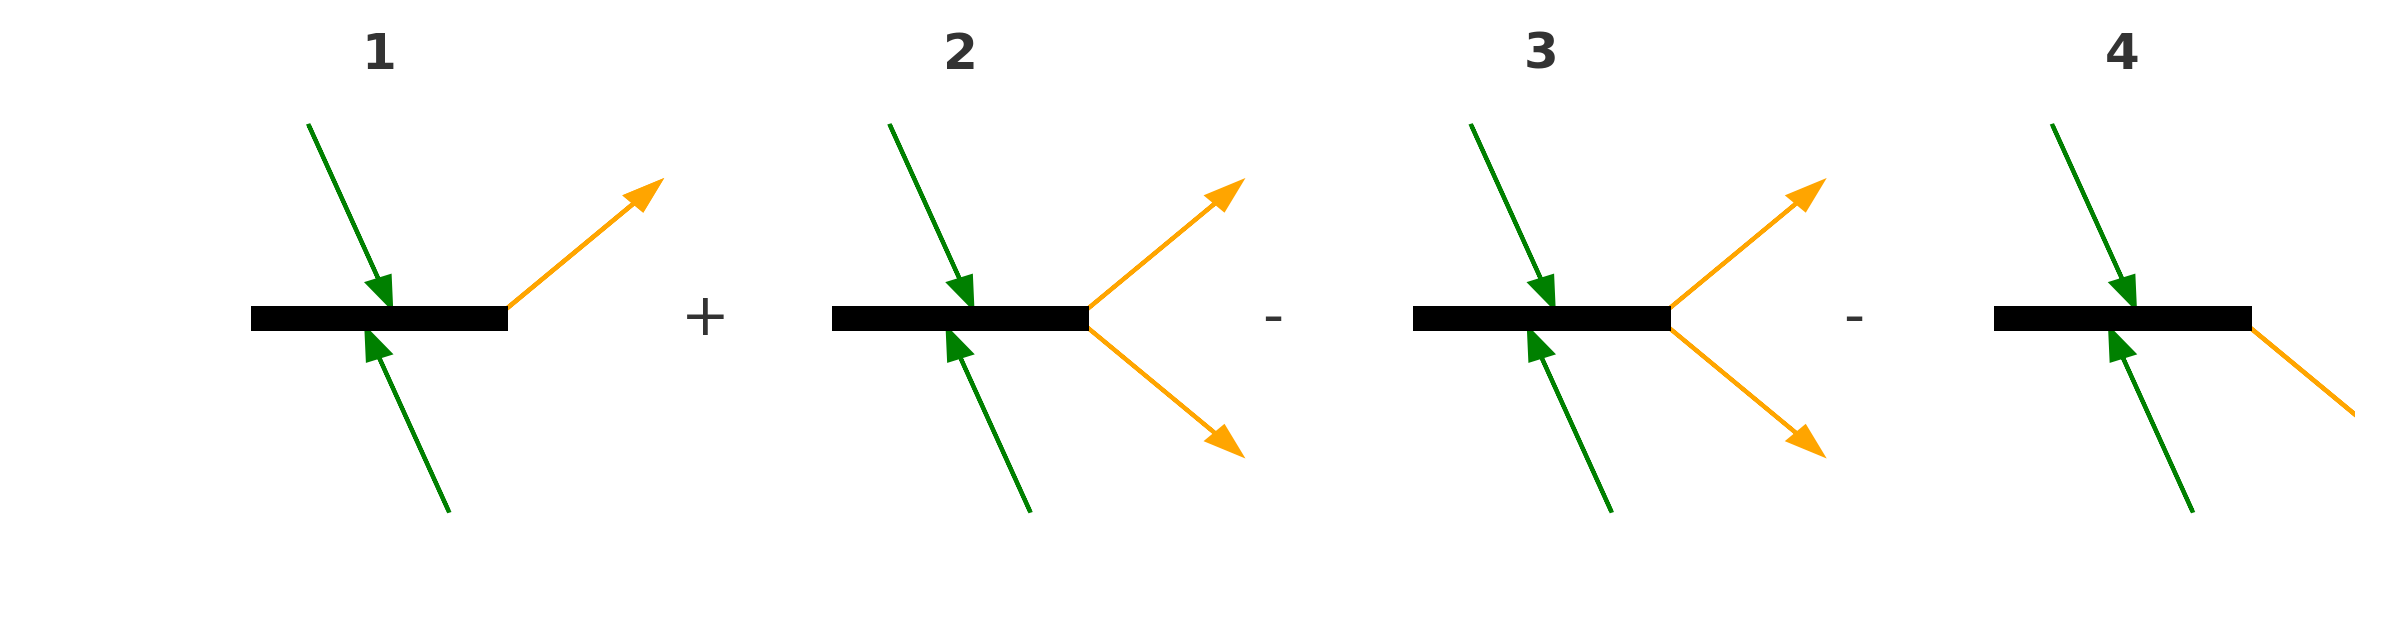
\includegraphics[width=0.95\textwidth]{bilder/hom_interferenzpfade_korrigiert.png}
	\end{center}
	\caption{Four possible paths of two photons at a beam splitter.\\
		The middle cases would lead to coincidence – but cancel due to interference.}
\end{figure}

\begin{tcolorbox}[hinweisbox, title=What This Diagram Shows]
	\label{box:was diese Darstellun}
	\small
	The diagram shows the four possible paths two identical photons can take when hitting a beam splitter.\\
	In cases 1 and 4 both photons exit together through the same output – exactly as observed experimentally.
	
	Paths 2 and 3 would lead to the photons arriving at different detectors (coincidence). But these cases cancel out due to destructive interference – because of the indistinguishability of the photons and the quantum-mechanical superposition of their amplitudes.
	
	The result: with perfect overlap both detectors are never triggered simultaneously – a clear sign of the quantum nature of light.
\end{tcolorbox}

According to classical expectation, each photon should be reflected or transmitted with 50% probability.\index{Reflection}\index{Transmission} But in quantum reality something different happens: both photons always leave through the same output – never opposite ones.

This phenomenon arises from the interference of the \emph{probability amplitudes} of the two processes. It shows: photons are indistinguishable and can interfere at the quantum level – not as fields, but as particles with wave nature.\index{Interference}\index{Photon Indistinguishability}

\vspace{1em}
\begin{tcolorbox}[physikbox, title=What the HOM Effect Shows]
	\label{box:HOM-Effekt}
	\small
	Two photons can “prevent” themselves from taking different paths – through the interference of their quantum states.\\
	This can only be explained if photons are considered indistinguishable quantum particles.
\end{tcolorbox}
\newpage
\noindent
\subsection{Conclusion}\index{Photoelectric Effect}\index{Compton Scattering}\index{Double-Slit Experiment}\index{Antibunching}\index{Hong–Ou–Mandel Effect}\index{Wave–Particle Duality}

\begin{tcolorbox}[hinweisbox, title=What the Experiments Show About Light]
	\label{box:was die Experimente}
	\small
	The four experiments discussed in this chapter – the photoelectric effect, Compton scattering, the double slit with single photons, and modern quantum experiments such as antibunching and the Hong–Ou–Mandel effect – demonstrate impressively that light cannot be explained by classical models alone.
	
	\begin{itemize}
		\item The \textbf{photoelectric effect} shows: light transfers \emph{energy} in discrete portions (photons).
		\item \textbf{Compton scattering} shows: photons also carry \emph{momentum} – like particles.
		\item The \textbf{double-slit experiment} shows: photons display \emph{wave patterns} in their distribution – even when occurring one at a time.
		\item \textbf{Antibunching} and the \textbf{Hong–Ou–Mandel effect} show: photons are \emph{indivisible}, \emph{non-classically indistinguishable}, and subject to the rules of quantum mechanics.
	\end{itemize}
	
	(A more detailed derivation of quantum interference at the beam splitter in the HOM effect can be found in Appendix~A, Section~\ref{anhangA:HOM}.) 
	
	Together these experiments prove: light is not an either–or of wave and particle – it is both at once, depending on the experiment. The photon concept is therefore not just a calculational tool – but physically real.
\end{tcolorbox}
